\documentclass{article}
\usepackage{amsmath, graphicx, amsfonts, caption, subfig, keyval}


% packages added LEO (remove algorithm, algorithmic)
\usepackage{xcolor}
\usepackage{hyperref}
\usepackage[boxruled,procnumbered, linesnumbered]{algorithm2e}
% packages added LEO end


\captionsetup{justification=centering}
\newcommand{\R}{\mathbb{R}}
\newcommand{\C}{\mathcal{C}}
\newcommand{\X}{\mathcal{X}}
\DeclareMathOperator*{\argmin}{\arg\!\min}

\begin{document}
\title{AM221 Final Project Proposal}
\author{Taylor Killian \& Leonhard Spiegelberg}
\maketitle

\begin{abstract}
To be filled with an interesting summary of our work and results

\end{abstract}

%% Leos thoughts

\section{Dictionary Learning as 2-stage supermodular minimzation}
The introduced problem of Dictionary learning, which in its general form can be seen as
\[
\min_{D, R, \theta, \lambda} f(D, R, X) + g(D, \theta) + h(R, \lambda)
\]
where $f$ describes the objective function used to measure goodness of approximation of $X$ through $D, R$, $g$ describing suitable constraints on the dictionary, $h$ on the representation respectively.
With an input dataset $X=[x_1, \dots, x_k],  x_i \in \R^d,  X \in \R^{d\times k}$ we wish to find a dictionary $D \in \R^{d\times n},  \mathcal{D} = [d_1, \dots, d_n]$ and a representation $\mathcal{R}=[r_1,\dots,r_k], \ r_i\in\R^n, \ \mathcal{R}\in\R^{n\times k}$, such that both $\|X-\mathcal{D}\mathcal{R}\|_F^2$ is minimized and the representations $r_i$ are "sparse enough". To limit the dictionary becoming infinitely large (or small) we introduce a constraint on the dictionary's columns. For this any sufficient norm can be used. An often used norm is the $l_2$-norm. 
Thus for the dictionary learning problem we introduce the problem with constraints
\begin{alignat}{5}
         &\min_{D, R} \|X \ -D R\|_F^2  & \quad   \\
         &\text{s.t.}  \quad  &\|d_j\|_2 \leq 1&, \forall j=1, ...,n  \quad \\
         &  \quad  &\|r_i\|_0 \leq t&, \forall i=1, ...,k  \quad 
\end{alignat}

\textcolor{red}{Description of constraints here}


Using Lagrange multipliers this can be brought to the general form above
\[
\min_{D, R, \theta, \lambda} \|X \ -D R\|_F^2 + \sum_{j=1}^m \theta_j (\| d_j\|_2 - 1)+ \sum_{i=1}^k \lambda_i (\| r_i \|_0 - t)
\]
I.e. the functions are
\[
\begin{split}
f(D, R, X) &:= \|X \ -D R\|_F^2 \\
g(D, \theta) &:= \sum_{j=1}^n \theta_j (\| d_j\|_2 - 1) \\
h(R, \lambda) &:= \sum_{i=1}^k \lambda_i (\| r_i \|_0 - t)
\end{split}
\]
\textcolor{red}{How to bring this to the penalty function form?}

The difficulty in solving this problem comes from the mathematical challenge the $\| . \|_0$ norm yields. To understand this better confer \autoref{fig:l012plot}.
\begin{figure}
\centering
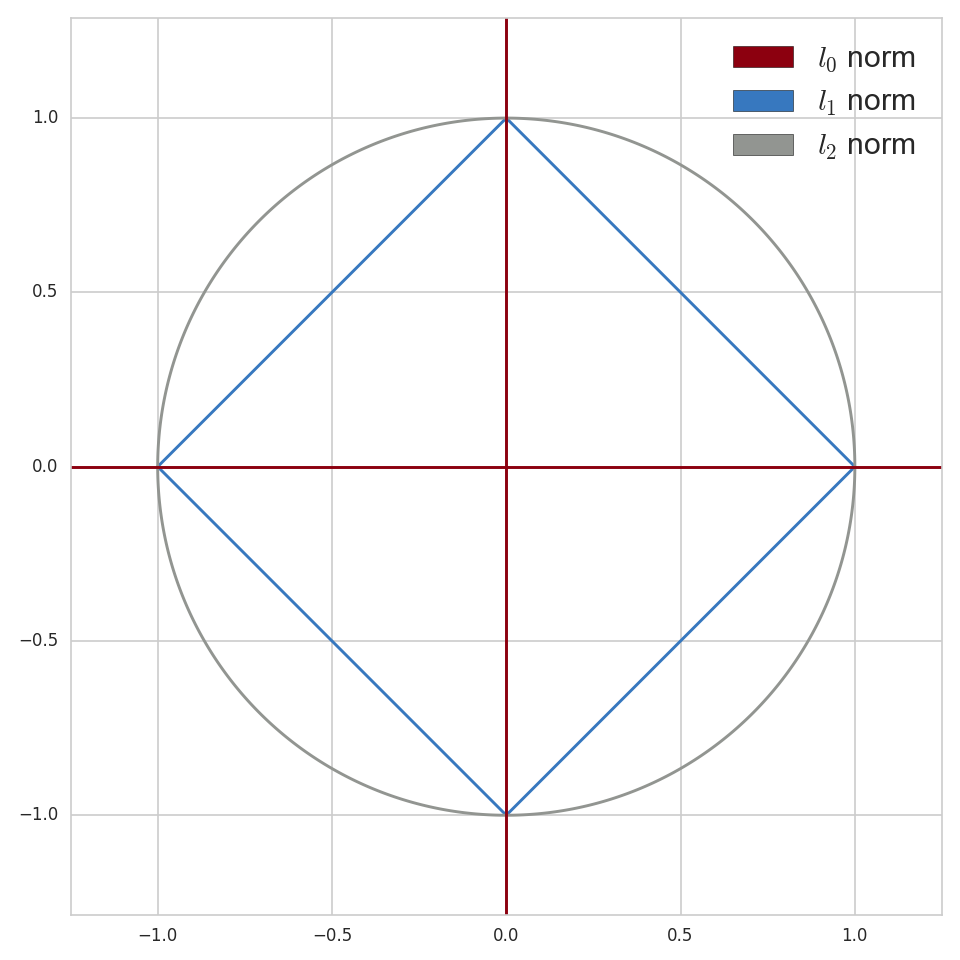
\includegraphics[scale=0.3]{img/l012_norms.png}
\caption{contour plot of the $l_0, l_1, l_2$ norm at levelset $L_1(f) := \lbrace x \in \R^2 : f(x) = 1 \rbrace $. Note that for any space $\R^d$, the image of the $l_0$ consists of $d+1$ values ($\lbrace 0, ..., d \rbrace $).}
\label{fig:l012plot}
\end{figure}
Let $x \in \R^d$
\[
l_0(x) := (\#i : x_i \not= 0)
\]
\textcolor{red}{here describe different norms...}
the goal is to find a norm that sort of converges to the infinite + of the l0 norm
\\

\textcolor{red}{Put here section about possible relaxations of l0 norm (related literature)}

\subsubsection{Two stage thoughts}
We will now relax the problem by formulating it into two stages:
\begin{enumerate}
\item solve for fixed $D, \theta$ the minimization to obtain optimal $R, \lambda$.
\item solve optimization for $D, \theta$ with obtained values
\item repeat previous steps until done
\end{enumerate}
\textcolor{red}{This is actually the method of optimal directions!}
In the traditional method of optimal directions (\textcolor{red}{ref here}) the subproblem $\min_{R, \lambda} f(D, R, X) + g(D, \theta) + h(R, \lambda)$ is solved either by various relaxation methods (i.e. LASSO, Matching Pursuit(\textcolor{red}{maybe describe here})), however for our approach we want to embedd the problem into a combinatorial optimization framework, which guarantees us bounds on optimality. Recent work done by \cite{weaklyalpha} showed that the subproblem of finding an optimal representation with a given dictionary is equivalent to Sparse Multiple Linear Regression (SMLR) and can be reformulated as a $\alpha$-weakly supermodular function. We will now show how to obtain this formulation:
Remember
\[
\begin{split}
\min_{R, \lambda} f(D, R, X) + g(D, \theta) + h(R, \lambda) \\
= \min_{R, \lambda} \|X -D R\|_F^2 + \sum_{j=1}^n \theta_j (\| d_j\|_2 - 1)+ \sum_{i=1}^k \lambda_i (\| r_i \|_0 - t)
\end{split}
\]
then let $S \subseteq [n]$ be a set of column indices for the dictionary. From now onwards we will assume that the given, fixed dictionary is normalized, i.e. $\forall d_i: \|d_i \|_2 = 1$. This allows us to remove the term $g(D, \theta)$. Define now $D_S$ as the matrix obtained from $D$ with all columns not indexed by $S$ to be set to zero.
\[
(D_S)_{ij} := \begin{cases}
0 \quad &j \notin S \\
D_{ij} \quad &j\in S
\end{cases}
\]

$D_S^+$ is the pseudoinverse which can be obtained i.e. via singular value decomposition when $D_S = U\Sigma V^T$ through $D_S^+ = V \Sigma^+ U^T$.
Then the problem can be equivalently stated as
\[
\begin{split}
 \min_{R, \lambda} \|X  -D R\|_F^2 + \sum_{i=1}^k \lambda_i (\| r_i \|_0 - t)\\
 \Longleftrightarrow 
  \min_{S \subseteq [n], |S| \leq t} \|X  -D_SD_S^+ X\|_F^2
 \end{split}
\]
\cite{weaklyalpha} have shown that the objective function $f(S) := \|X  -D_SD_S^+ X\|_F^2$ of this optimization problem is $\alpha$-weakly supermodular with 
\[ 
\alpha = \max_{\tilde{S} \subseteq [n]}\| D_{\tilde{S}}^+ \|_F^2
\]

\subsection{How to combine it}
For the two stage formulation we can generally think of the problem as of adapting the idea of the method of optimal directions but instead of projecting the given representation onto the dictionary we strive for an additional minimization problem:
Let $f_1, ..., f_m$ be instances of the SMLR problem with different dictionaries $D_k$
\[
f_k := \min_{D_k, R, \lambda} \|X  -D_k R\|_F^2 + \sum_{i=1}^k \lambda_i (\| r_i \|_0 - t)
\]
 Then the dictionary problem can be seen as
\[
\min_{D, \theta} q(f_1, ..., f_m) + \sum_{j=1}^n \theta_j (\| d_j\|_2 - 1)
\]
for some combination function $q$. We now ask, which properties such a combination function ideally should satisfy.
\\
\textcolor{red}{that is a great question! Can we formulate some ideas, thoughts on what it should look like? I am still unsure about the above formulation...}
 \\
 One choice for $q$ could be 
 \[q(f_1(D, \theta), ..., f_m(D, \theta)) := \sum_{i=1}^m f_i(D, \theta)\]
  another one to minimize the product of the SMLR instances. Reformulating it with a logarithm might give even better results with increased computationally tractability 
 \[
 q(f_1(D, \theta), ..., f_m(D, \theta)) = \sum_{i=1}^m \log (f_i(D, \theta))
 \]
 (\text{red}{we can omit the logical step of log'ing also the lambda term because it is a constraint...})
 
 \subsubsection*{Algorithm proposals}
 In the following we proprose a general randomized greedy algorithm to solve the dictionary learning problem.
 
 \begin{centering}
\begin{algorithm}[H]
\SetKwData{Left}{left}
\SetKwData{This}{this}
\SetKwData{Up}{up}
\SetKwFunction{RandomDict}{RandomDictionary}
\SetKwFunction{alphaSup}{$\alpha$-GreedySolver}
\SetKwInOut{Input}{input}\SetKwInOut{Output}{output}

\Input{A data matrix $X \in \R^{d \times k}$}
\Output{A dictionary $D \in \R^{d \times n}$ and representation $R \in \R^{n \times k}$}

$D_0 \gets$ \RandomDict{$-1$, $1$} \tcp*[f]{assert $D_0 \not= 0$} \\
normalize s.t. $\| (D_0)_{*j}\|_2 = 1$\\
$S_0, R_0 \gets $ \alphaSup{$X$, $D$, $t$}\\
$m \gets 0$\\
 \While{$m < \mathrm{MAXSTEPS}$ }{
 	$D_{m+1} \gets X_{S_m \setminus \lbrace q\rbrace \cup \lbrace p\rbrace}$\\
	normalize s.t. $\| (D_{m+1})_{*j}\|_2 = 1$\\
	$S, R \gets $ \alphaSup{$X$, $D_{m+1}$, $t$} \\
	\If{$\| X - D_{m+1}R\|_F^2 < \| X - D_mR_m\|_F^2$} {
		$S_{m+1}, R_{m+1}  \gets S, R$
	}
	$m \gets m + 1$\\
  }
 \caption{General randomized greedy algorithm for Sparse Dictionary Learning}
 \label{algo:randgeneral}
\end{algorithm}
\end{centering}
We start by initializing a random dictionary that is non-zero. To allow for all directions negative and positive values should be picked. To restrict the dictionary size, normalization along columns is done in lines $2$ and $8$. We use the greedy algorithm as proposed in \cite{alphaweakly} to solve for a given dictionary the SMLR problem by using $t$ steps (yielding $t$ columns for representation). The indices of the columns that best solve the SMLR are returned as set $S$ along a representation $R$. We then iteratively refine the solution. Therefore one observation is crucial: Given a set of columns $S$ that represents the indices of non-zero columns of $R$, only $|S|$ corresponding columns in $D$ obtained through matrix multiplication will contribute something to the norm. Thus, in order to improve the solution we need to exchange one (or more) columns of the current set $S$ with some other column that might give a better solution. To obtain a new dictionary candidate we construct it by using a similar argument via the data matrix $X$. I.e. choose randomly a column index $q \in S$ that will be removed and add another random column index $p \in \lbrace 1, ..., k \rbrace \setminus S$. This step is performed in line 7, \autoref{algo:randgeneral}. We then obtain the dictionary candidate by $l_2$-column normalization and solve the resulting SMLR problem via the $alpha$-weakly supermodular greedy algorithm. If the new solution is better than the old one, we keep it, else we perform another round of local search.



\bibliographystyle{plain}
\bibliography{bibliography}

\end{document}